% !TEX encoding = UTF-8
% !TEX TS-program = pdflatex
% !TEX root = ../tesi.tex

\chapter{Fast-Broadcast}
	The previous work \cite{ROM2017} utilized a version of Fast-Broadcast in which vehicles having origin-vehicle distance smaller than origin-sender distance suppressed their transmission since they do not contribute in the outward propagation of the transmission. In the following graphs, the old version will be called \textit{TD-Fast-Broadcast} (as in \textit{Triangular-Distance-Fast-Broadcast}). The aim of this appendix is to show the reasons why this additional check has been removed in the version of the Fast-Broadcast algorithm used in this work thanks to simulations which employed two scenarios. More in detail, the aim of these simulations has been twofold:
	\begin{itemize}
		\item show that TD-Fast-Broadcast performs worse than Fast-Broadcast in terms of delivery ratios in difficult scenarios with buildings, particularly the Padua urban scenario;
		\show show that Fast-Broadcast is non-pejorative in all metrics in scenarios where TD-Fast-Broadcast did not show delivery ratio problems, such as the Los Angeles urban scenario.
	\end{itemize}

	\section{Fast-Broadcast's improvement on delivery ratios}
		\begin{figure}[H]
			\centering
			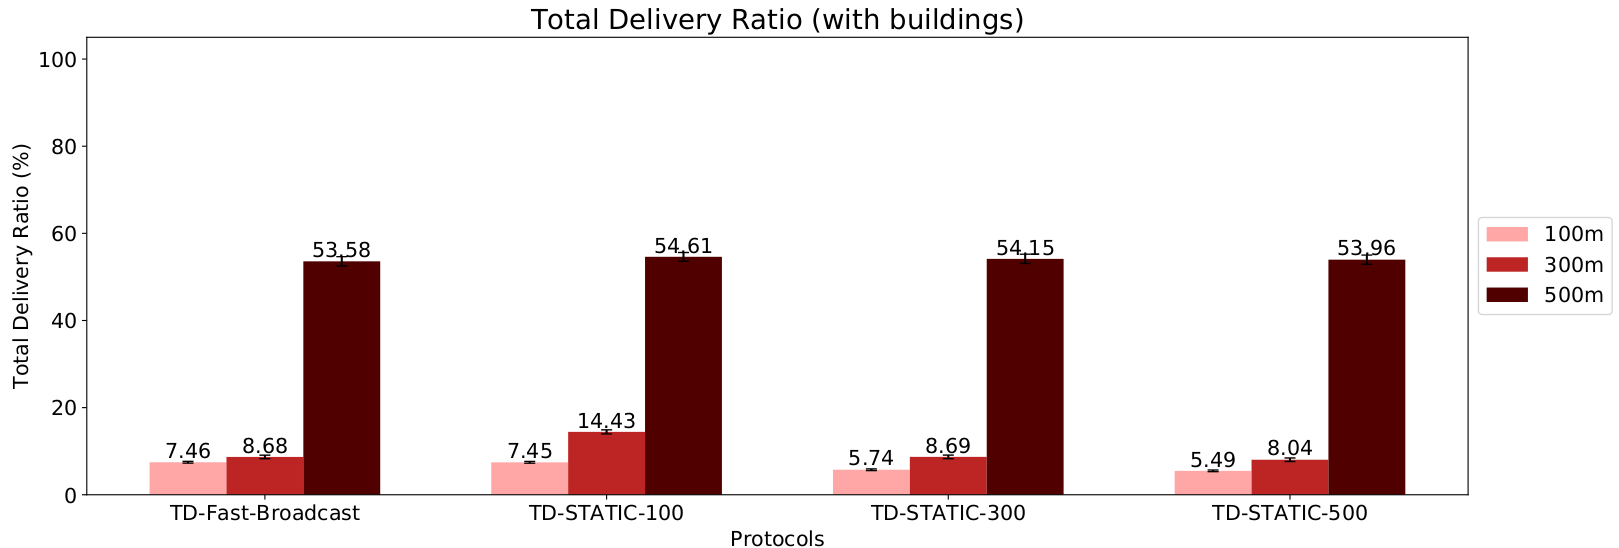
\includegraphics[width=1.0\textwidth]{immagini/td-fb-pd/td-fb/tdr}
			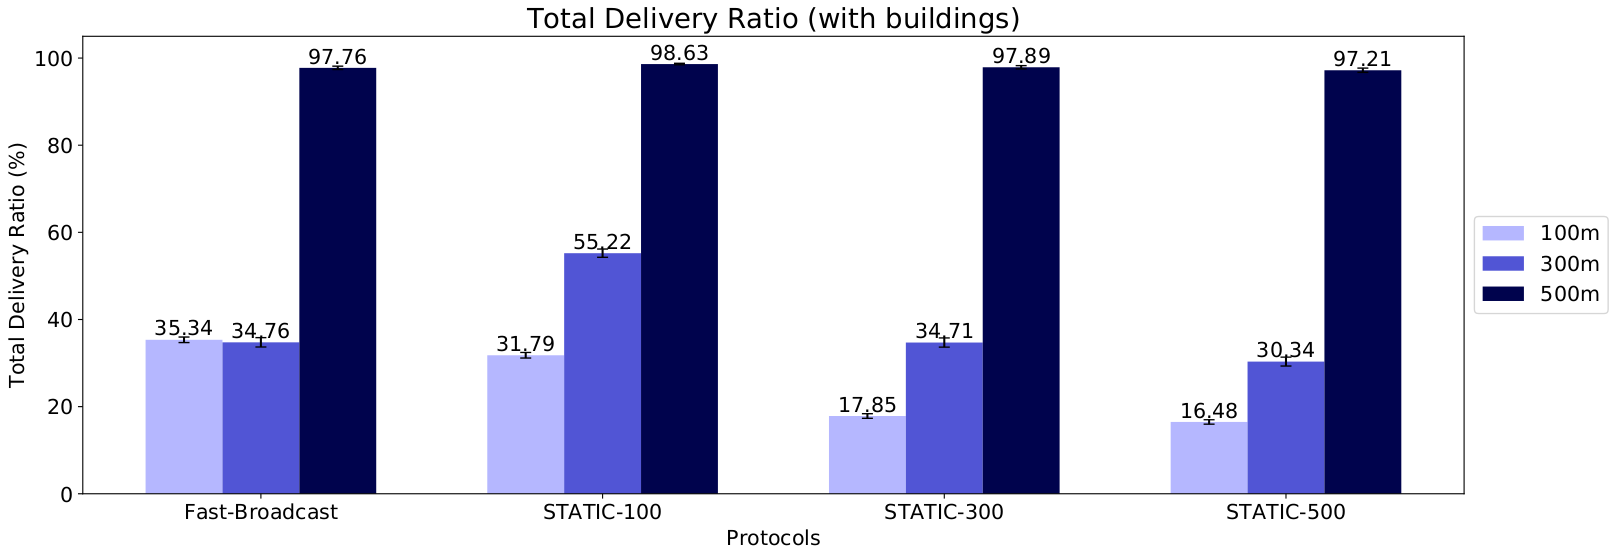
\includegraphics[width=1.0\textwidth]{immagini/td-fb-pd/fb/tdr}
			\caption{\textit{TDR} for TD-Fast-Broadcast (top) and Fast-Broadcast (bottom) for Padua urban scenario
			\label{fig:td-tdr}
		\end{figure}
	
		\begin{figure}[H]
			\centering
			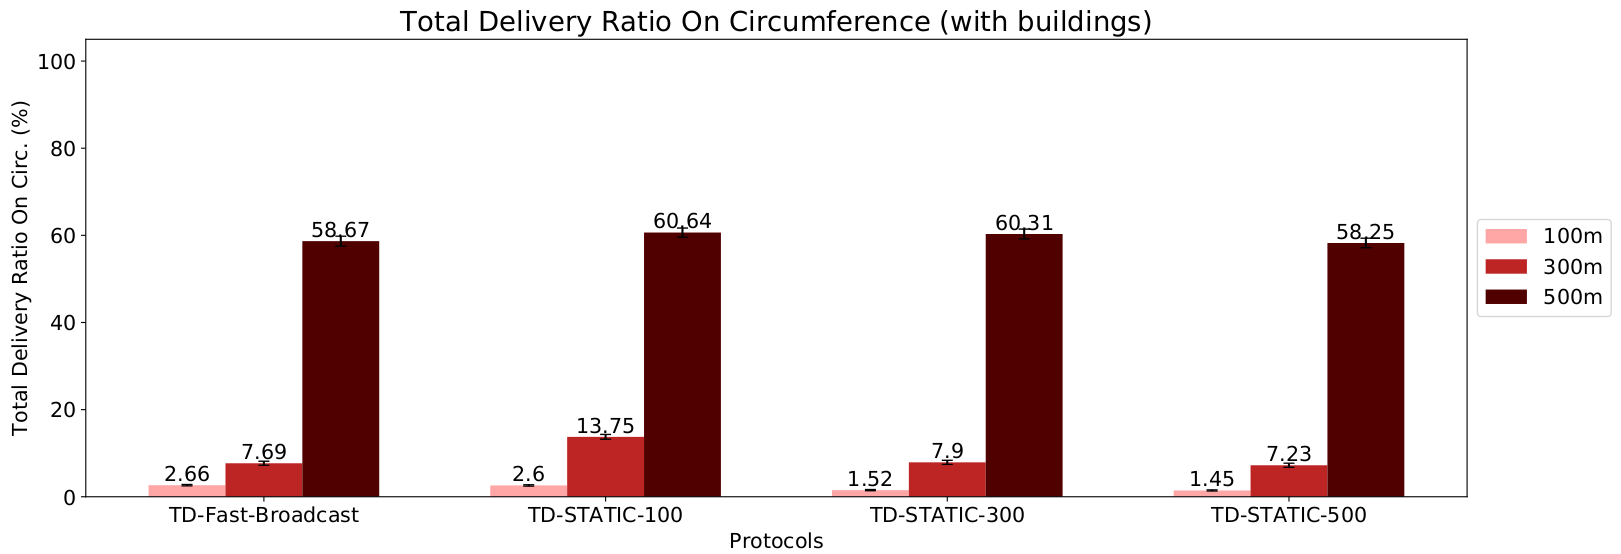
\includegraphics[width=1.0\textwidth]{immagini/td-fb-pd/td-fb/tdroc}	
			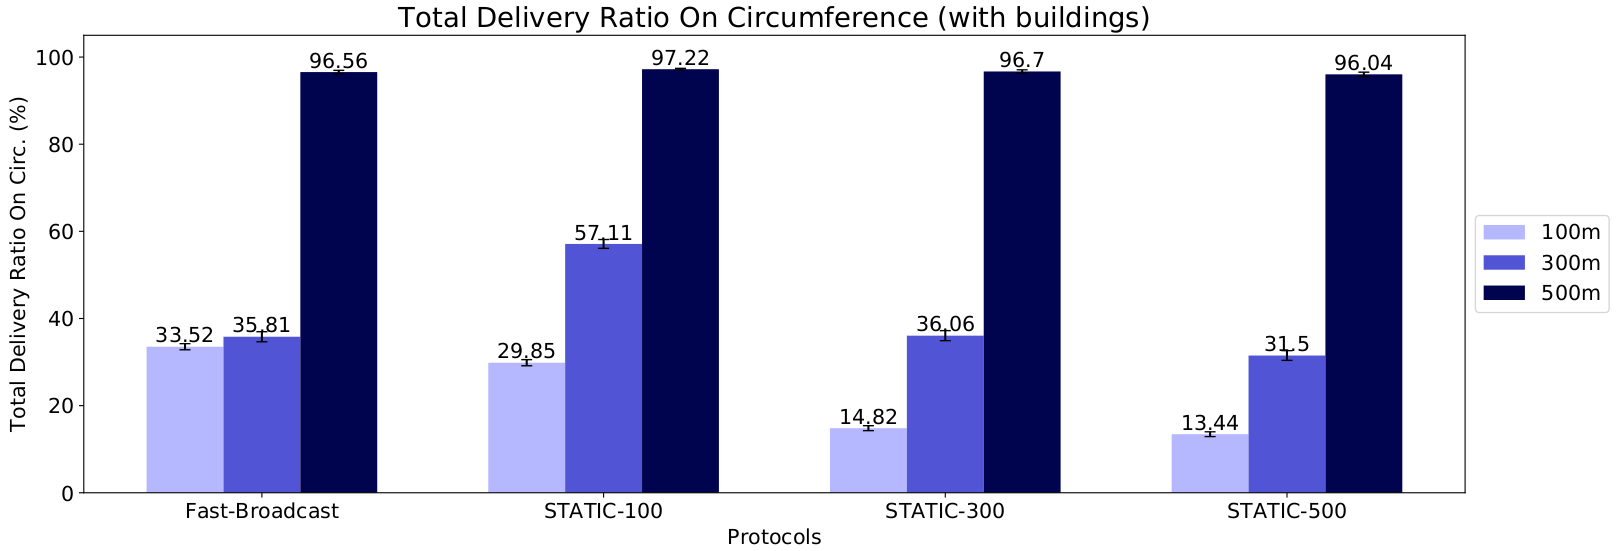
\includegraphics[width=1.0\textwidth]{immagini/td-fb-pd/fb/tdroc}
			\caption{\textit{TDROC} for TD-Fast-Broadcast (top) and Fast-Broadcast (bottom) for Padua urban scenario
			\label{fig:td-tdroc}
		\end{figure}
	
		\begin{figure}[H]
			\centering
			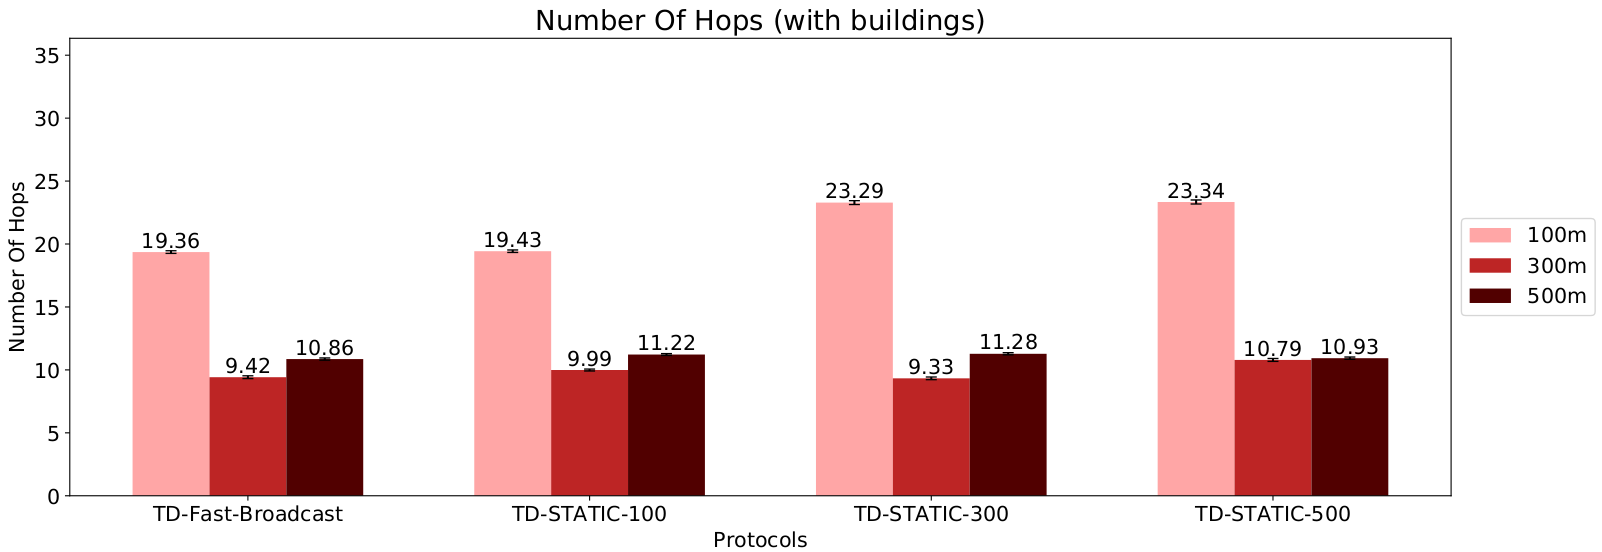
\includegraphics[width=1.0\textwidth]{immagini/td-fb-pd/td-fb/noh}	
			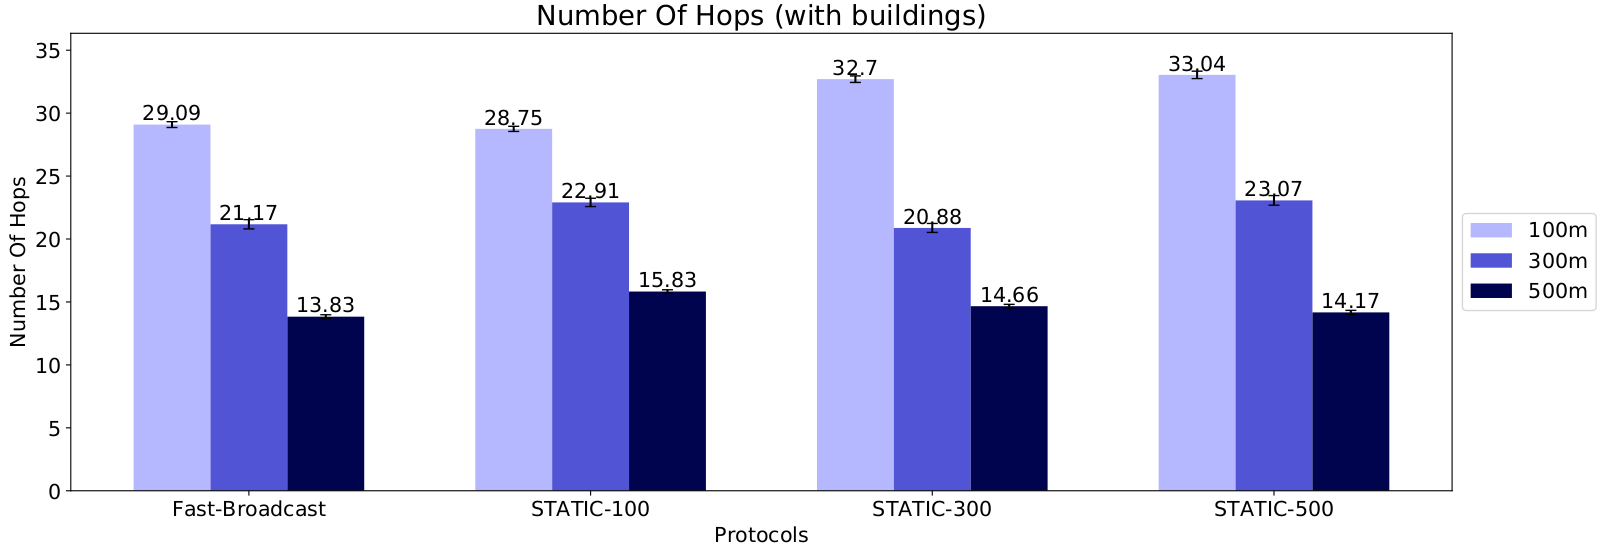
\includegraphics[width=1.0\textwidth]{immagini/td-fb-pd/fb/noh}
			\caption{\textit{NOH} for TD-Fast-Broadcast (top) and Fast-Broadcast (bottom) for Padua urban scenario
			\label{fig:td-noh}
		\end{figure}
	
		\begin{figure}[H]
			\centering
			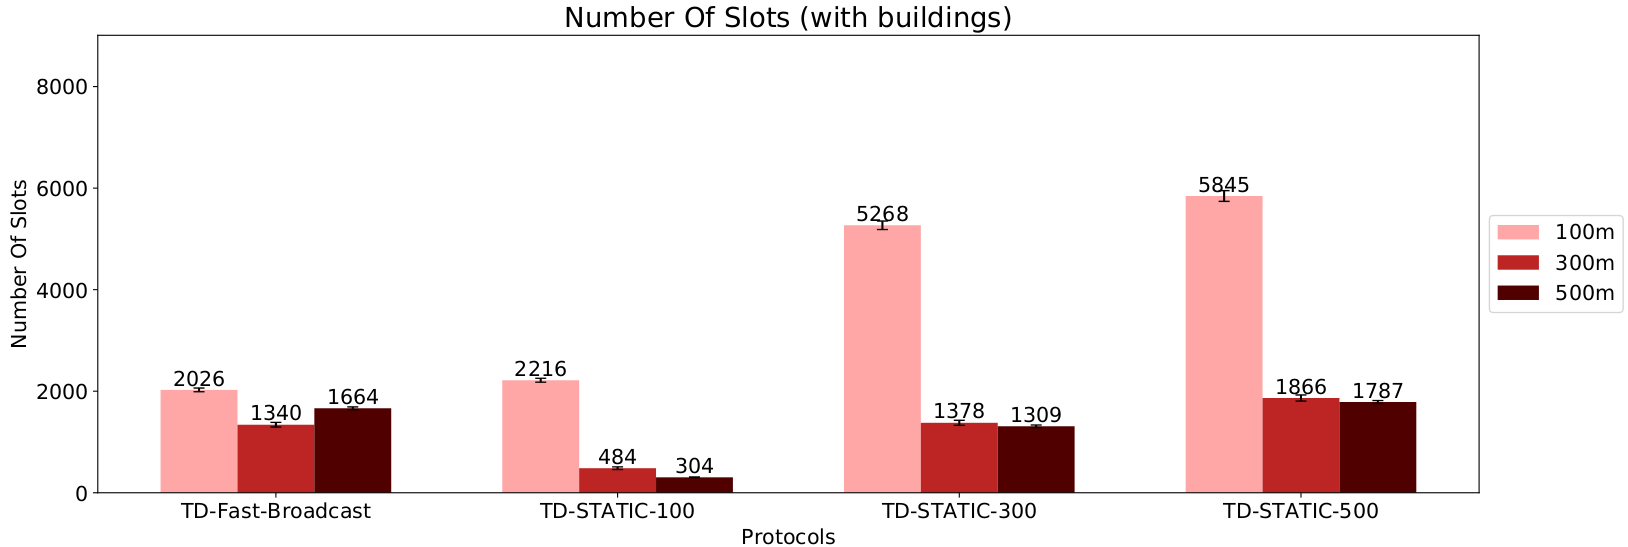
\includegraphics[width=1.0\textwidth]{immagini/td-fb-pd/td-fb/nos}	
			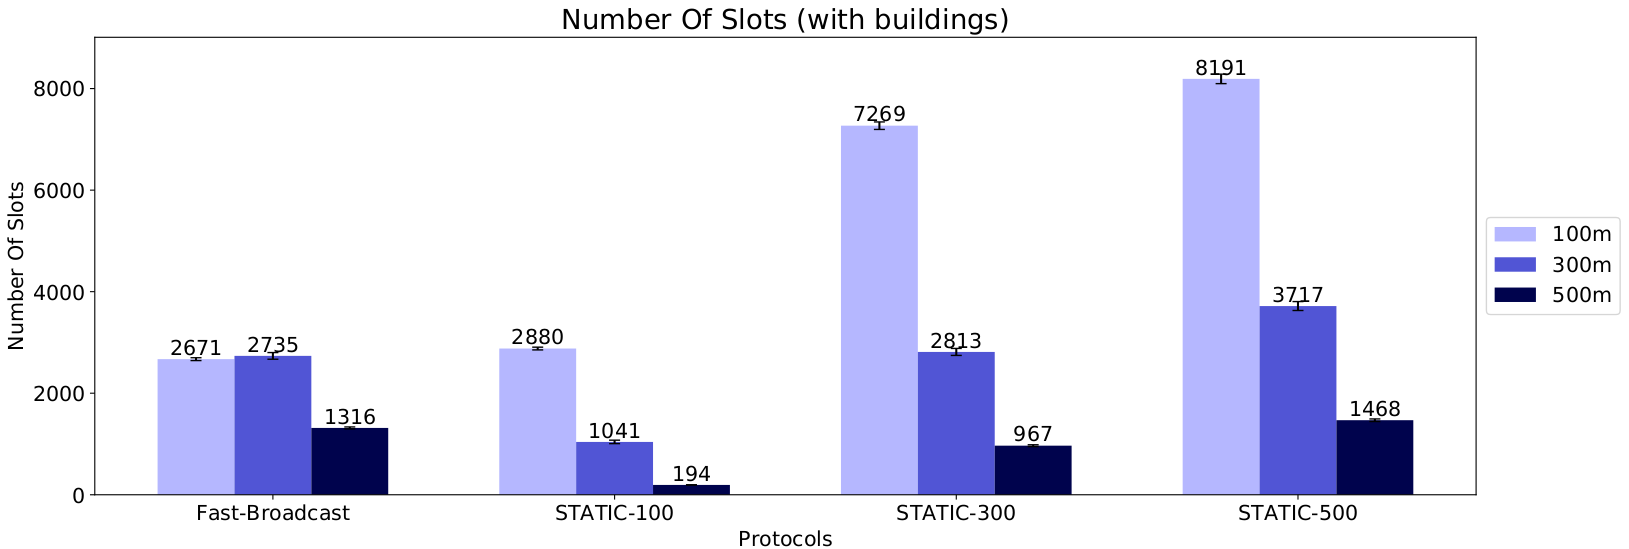
\includegraphics[width=1.0\textwidth]{immagini/td-fb-pd/fb/nos}
			\caption{\textit{NOS} for TD-Fast-Broadcast (top) and Fast-Broadcast (bottom) for Padua urban scenario
			\label{fig:td-nos}
		\end{figure}
		
		\begin{figure}[H]
			\centering
			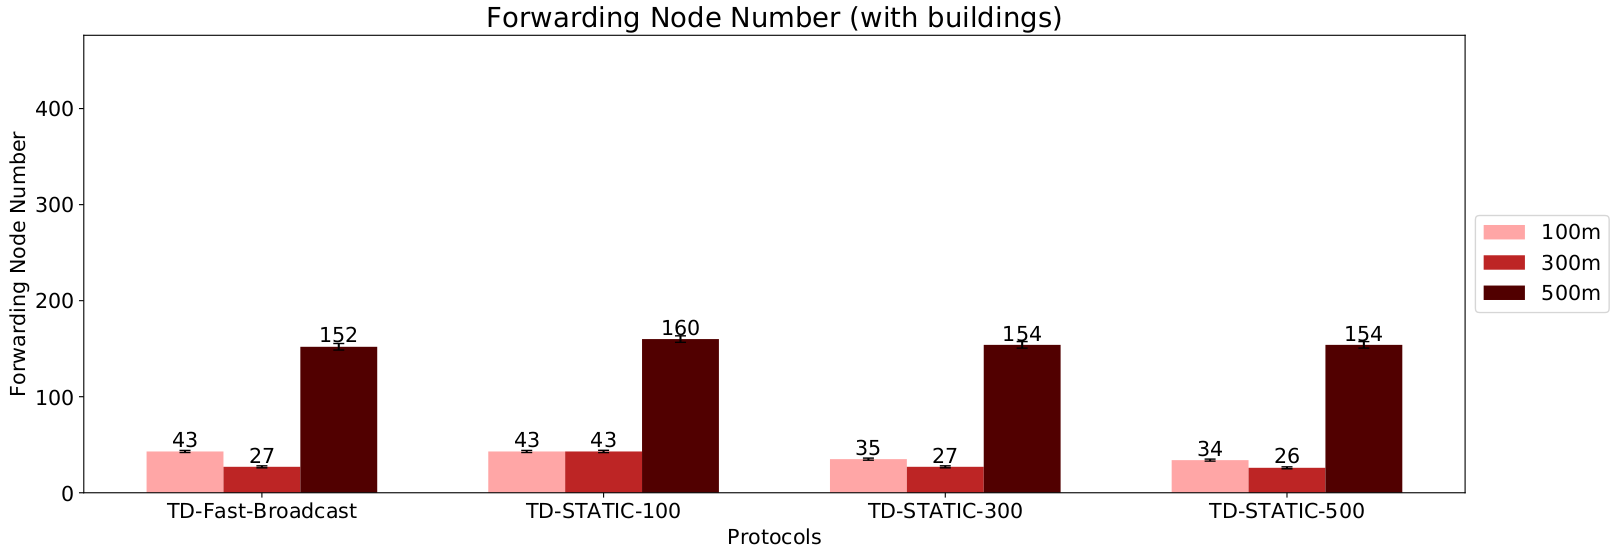
\includegraphics[width=1.0\textwidth]{immagini/td-fb-pd/td-fb/fnn}	
			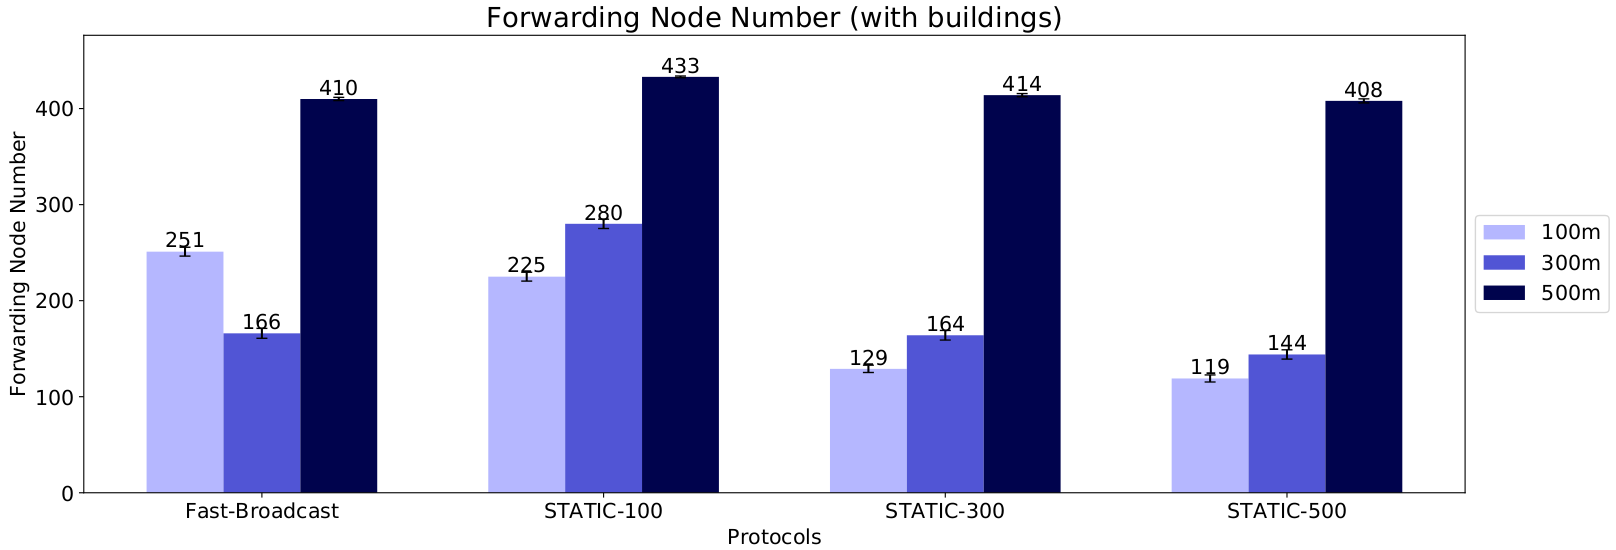
\includegraphics[width=1.0\textwidth]{immagini/td-fb-pd/fb/fnn}
			\caption{\textit{FNN} for TD-Fast-Broadcast (top) and Fast-Broadcast (bottom) for Padua urban scenario
			\label{fig:td-fnn}
		\end{figure}


	\section{Fast-Broadcast's non-pejorative effects}
		\begin{figure}[H]
			\centering
			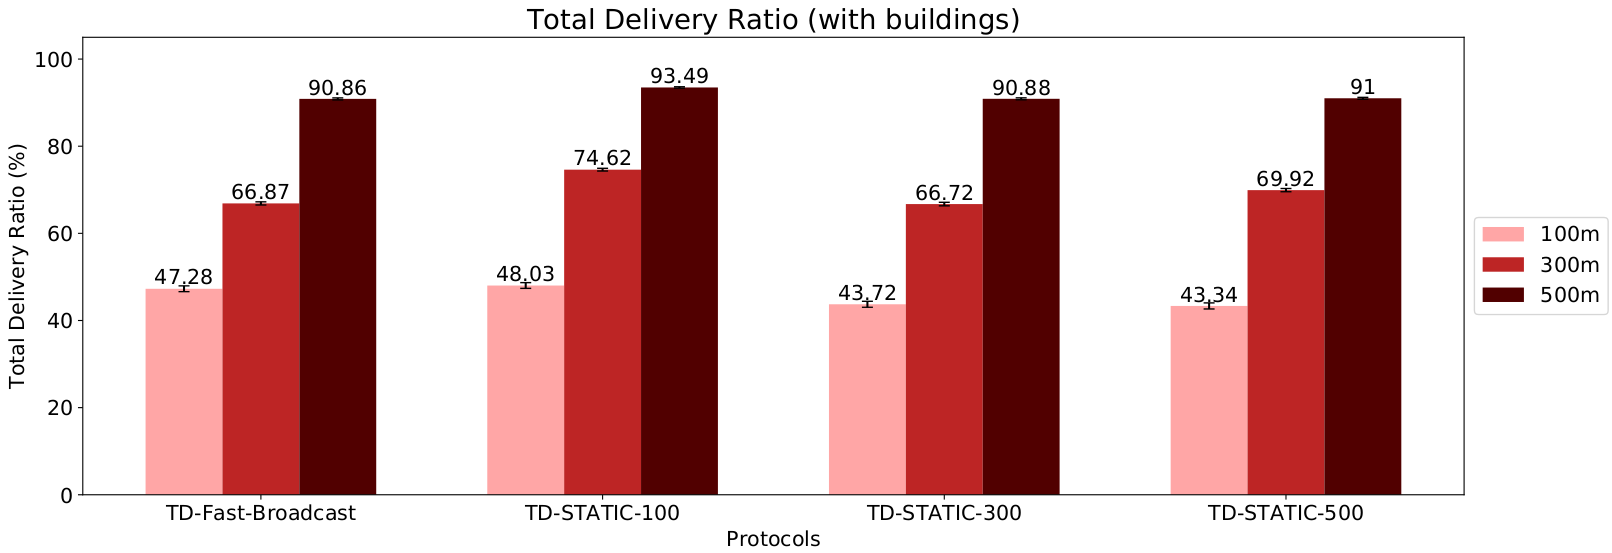
\includegraphics[width=1.0\textwidth]{immagini/td-fb-la/td-fb/tdr}
			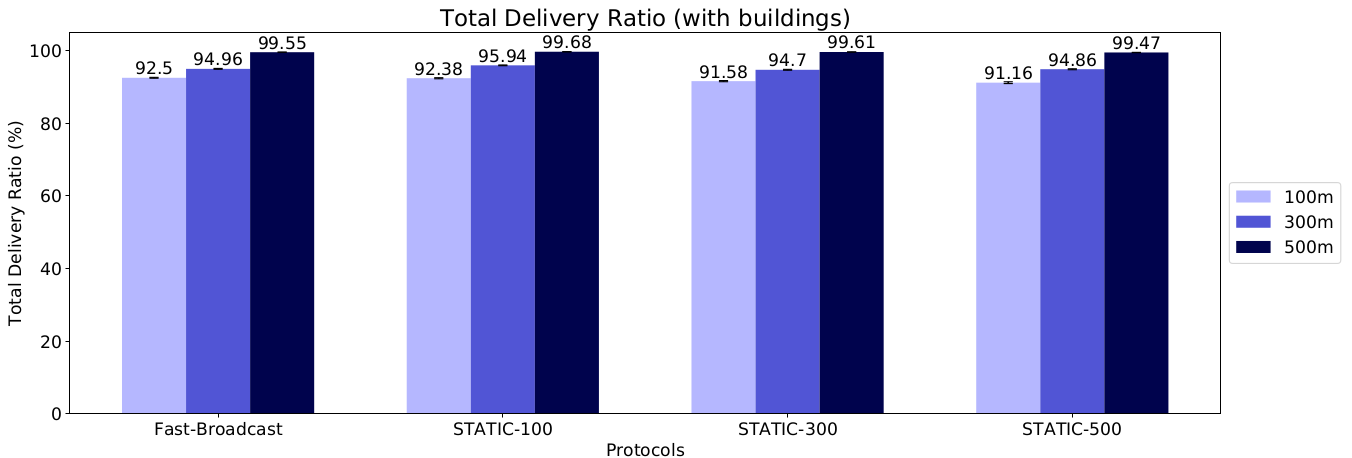
\includegraphics[width=1.0\textwidth]{immagini/td-fb-la/fb/tdr}
			\caption{\textit{TDR} for TD-Fast-Broadcast (top) and Fast-Broadcast (bottom) for Los Angeles urban scenario
			\label{fig:la-td-tdr}
		\end{figure}
			
		\begin{figure}[H]
			\centering
			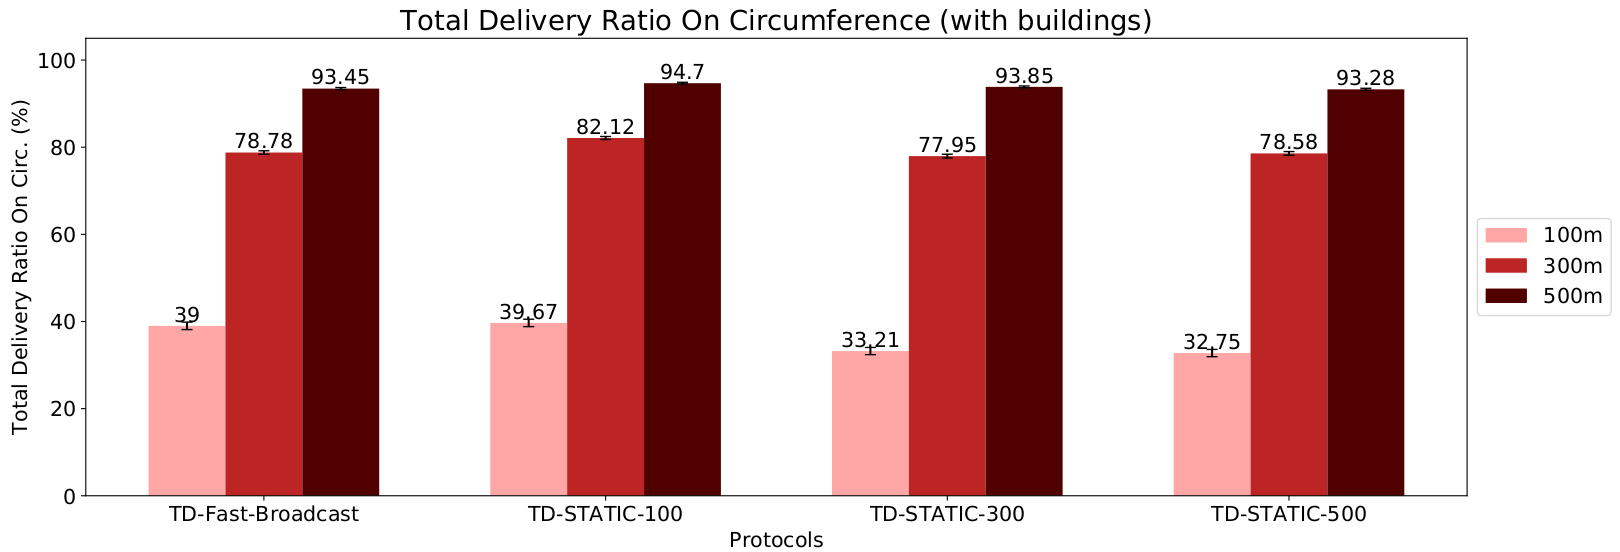
\includegraphics[width=1.0\textwidth]{immagini/td-fb-la/td-fb/tdroc}	
			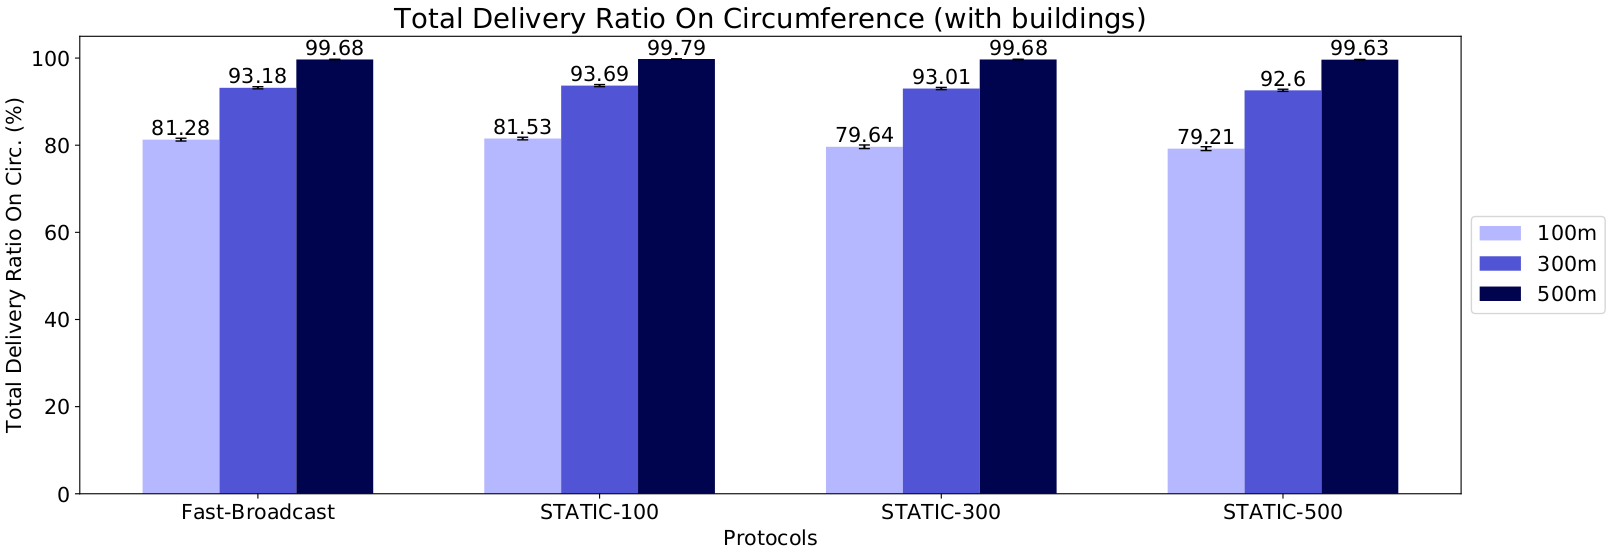
\includegraphics[width=1.0\textwidth]{immagini/td-fb-la/fb/tdroc}
			\caption{\textit{TDROC} for TD-Fast-Broadcast (top) and Fast-Broadcast (bottom) for Los Angeles urban scenario
			\label{fig:la-td-tdroc}
		\end{figure}
				
		\begin{figure}[H]
			\centering
			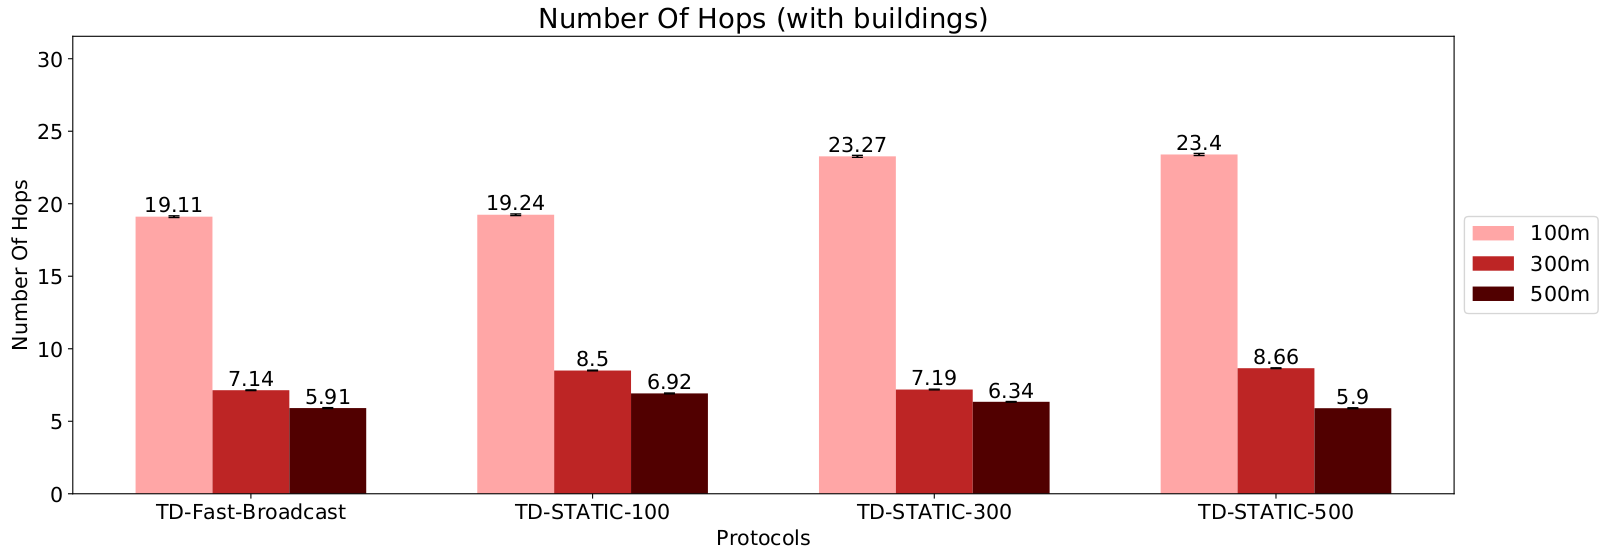
\includegraphics[width=1.0\textwidth]{immagini/td-fb-la/td-fb/noh}	
			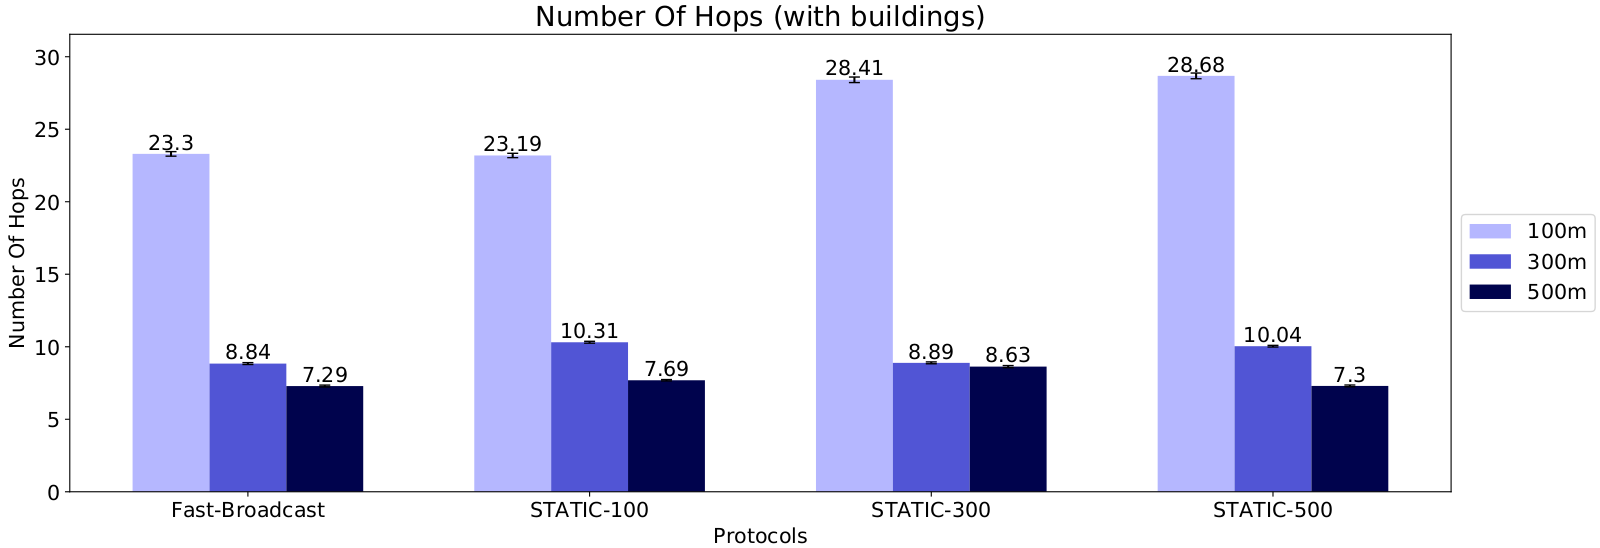
\includegraphics[width=1.0\textwidth]{immagini/td-fb-la/fb/noh}
			\caption{\textit{NOH} for TD-Fast-Broadcast (top) and Fast-Broadcast (bottom) for Los Angeles urban scenario
			\label{fig:la-td-noh}
		\end{figure}
					
		\begin{figure}[H]
			\centering
			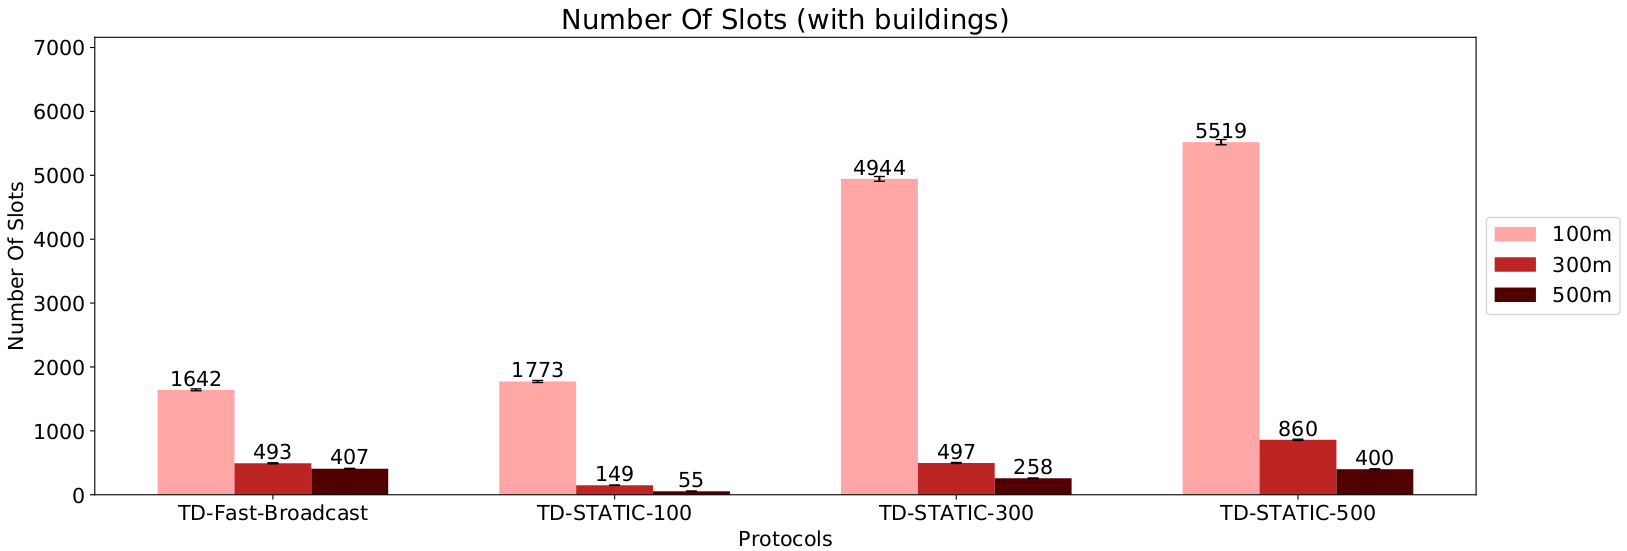
\includegraphics[width=1.0\textwidth]{immagini/td-fb-la/td-fb/nos}	
			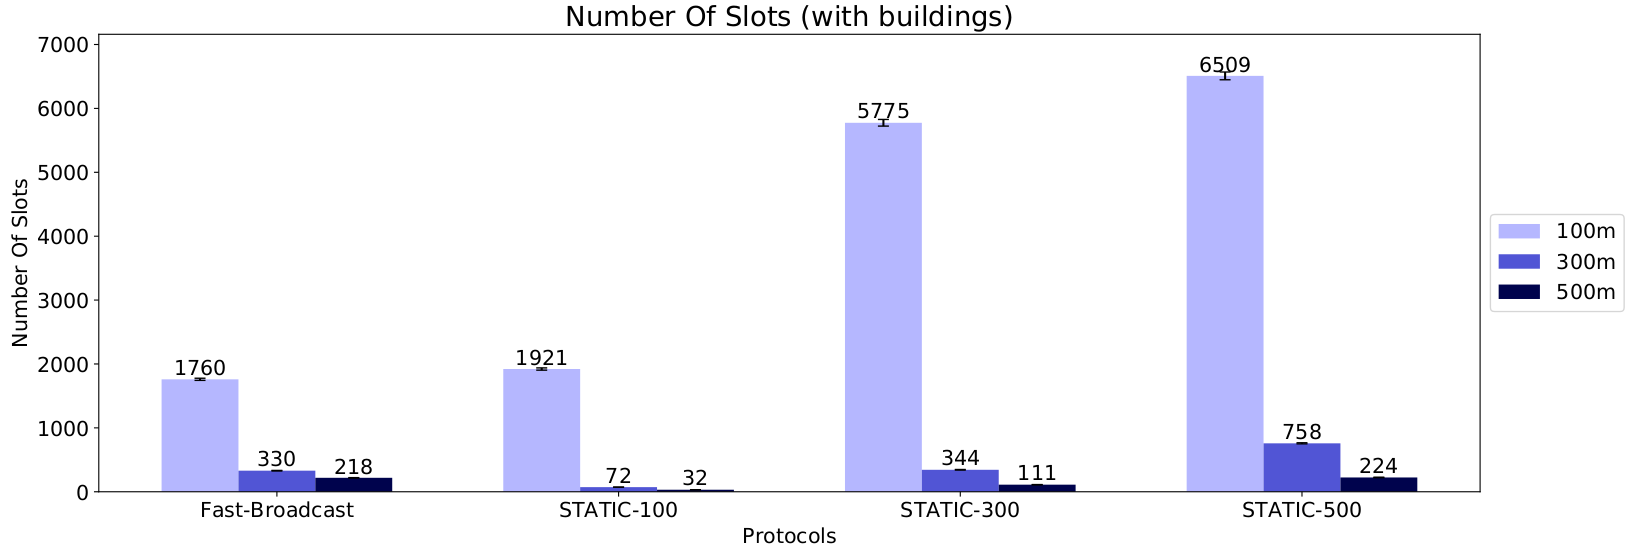
\includegraphics[width=1.0\textwidth]{immagini/td-fb-la/fb/nos}
			\caption{\textit{NOS} for TD-Fast-Broadcast (top) and Fast-Broadcast (bottom) for Los Angeles urban scenario
			\label{fig:la-td-nos}
		\end{figure}
						
		\begin{figure}[H]
			\centering
			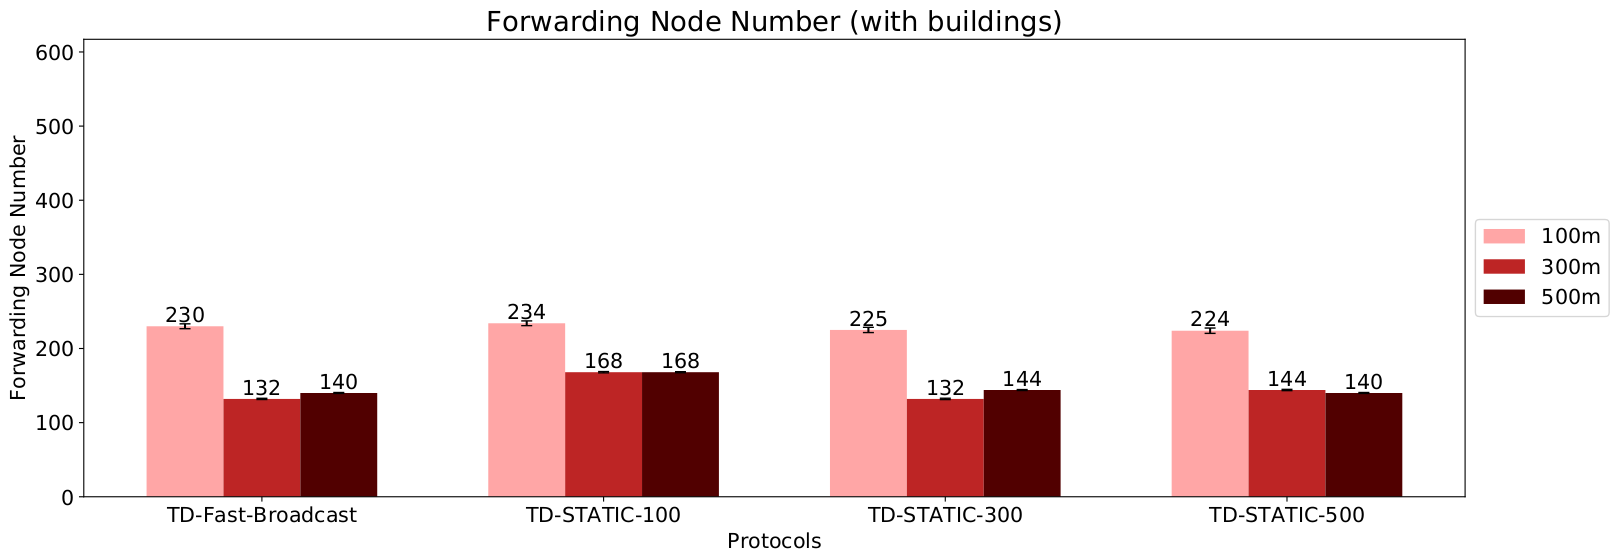
\includegraphics[width=1.0\textwidth]{immagini/td-fb-la/td-fb/fnn}	
			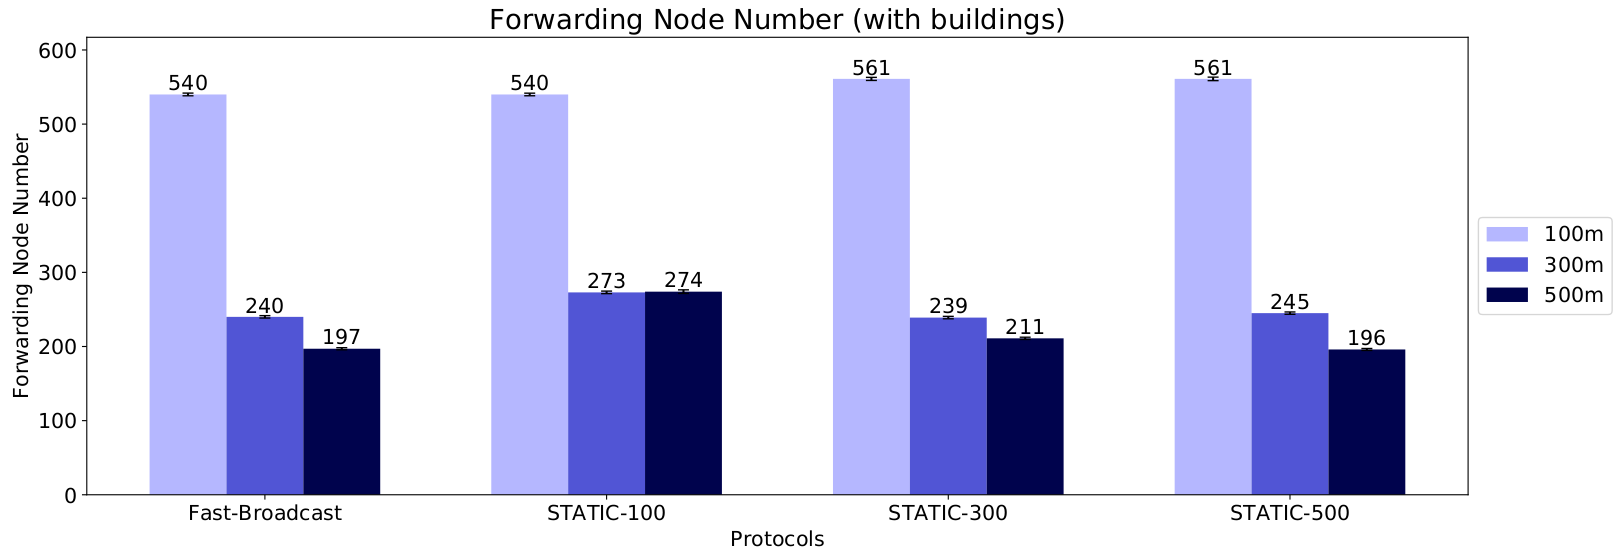
\includegraphics[width=1.0\textwidth]{immagini/td-fb-la/fb/fnn}
			\caption{\textit{FNN} for TD-Fast-Broadcast (top) and Fast-Broadcast (bottom) for Los Angeles urban scenario
				\label{fig:la-td-fnn}
		\end{figure}
		